\section{Sharding.}
Levantamos cinco shards siguiendo las instrucciones del archivo tutorial\_sharding.txt.

Luego creamos un indice simple sobre el atributo codigo\_postal.

Luego importamos el código de insert\_data.js donde tenemos
funciones que nos permiten ingresar datos de a 20k y pedir las estadísticas.
Finalmente, nos guardamos las estadísticas en archivos .txt. Los mismos se encuentran en
la carpeta mediciones.

\begin{figure}[H]
\centering
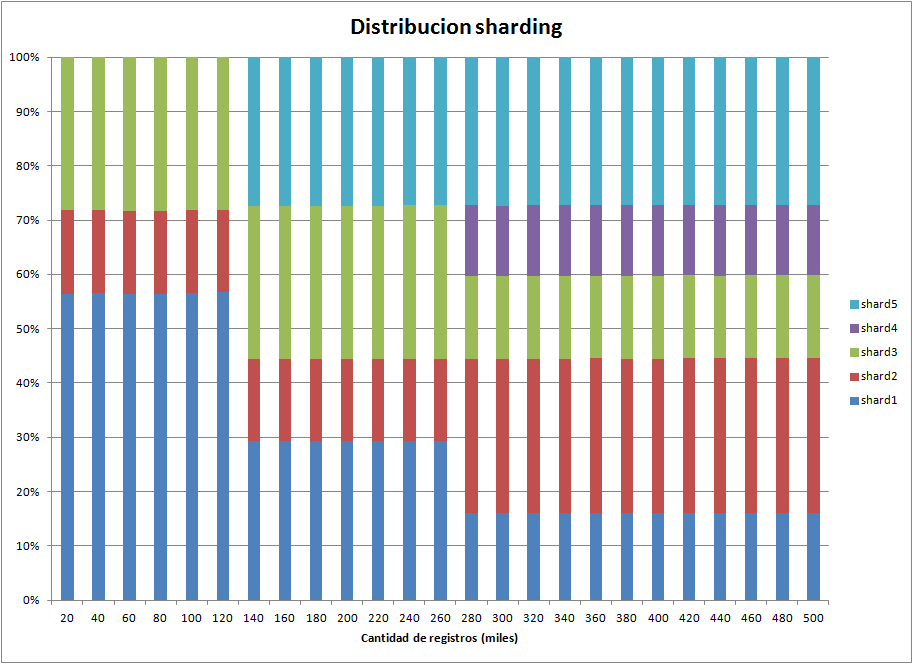
\includegraphics[width=165mm]{../mediciones/sharding_simple.png}
\caption{Porcentaje de distribucion entre los shards usando un
indice simple en base al codigo postal.}
\end{figure}

\begin{figure}[H]
\centering
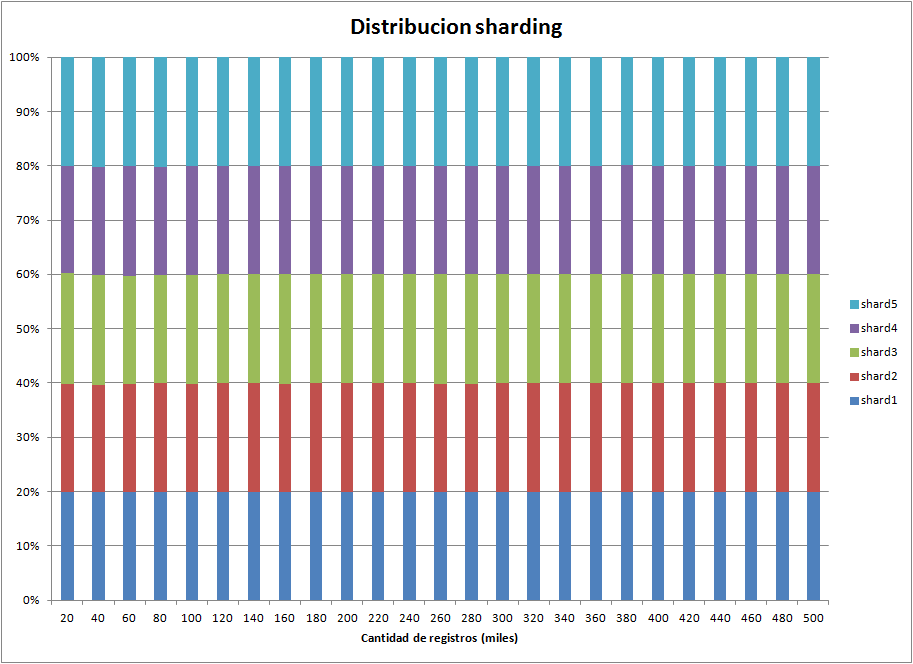
\includegraphics[width=165mm]{../mediciones/sharding_hashed.png}
\caption{Porcentaje de distribucion entre los shards usando un
indice hasheado en base al \_id}
\end{figure}


